%-----------------------------------------------------------------------------
\section{Three-phase structure of the Field}\label{sect:3BB}
%-----------------------------------------------------------------------------

  The total volume probability distributions for gas number density $n$, 
  temperature $T$ and thermal pressure $p$ are displayed in Fig.~\ref{fig:pdfm}
  from Models~$\Ompa$ (black, solid) and $\Omph$ (blue, dashed). 
%  Note that Model~$\Omph$ includes the correction to the SN distribution,
%  which stabilises the disc against unphysical cyclic oscillations, although
%  it is still subject to natural random vertical fluctuations.
%  Hence the mean density in the SN active region remains consistently higher
%  than in Model~\Op.
%-----------------------------------------------------------------------------
  \begin{figure}
  \centering
  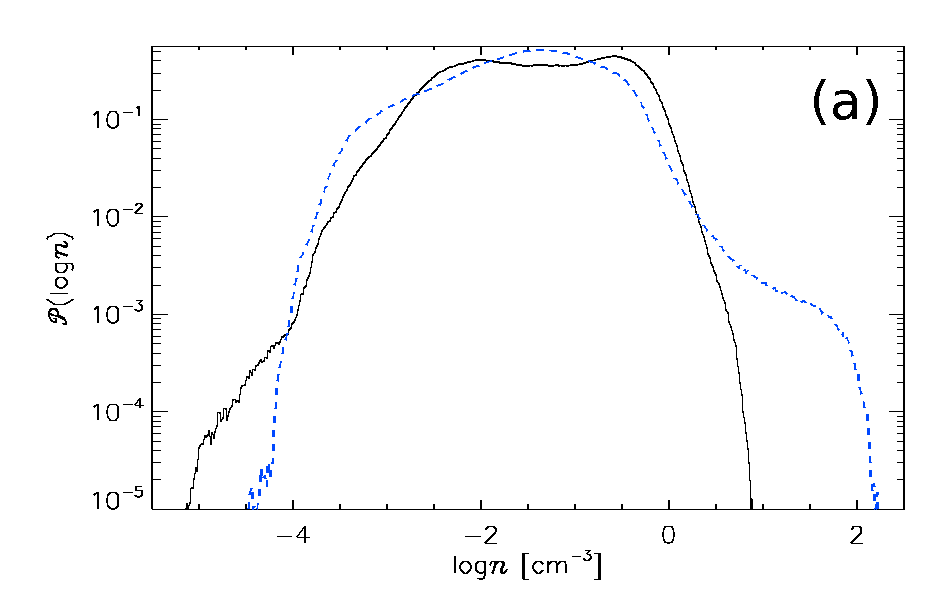
\includegraphics[width=0.9\columnwidth,clip=true,trim=0 0 0 9mm]{fig/o1pr_rpdf.png}
  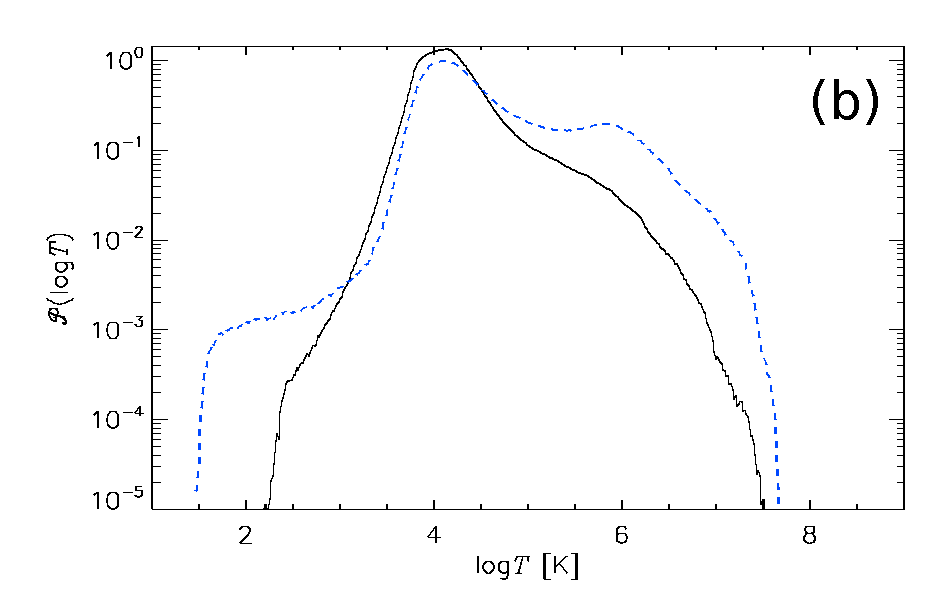
\includegraphics[width=0.9\columnwidth,clip=true,trim=0 0 0 9mm]{fig/o1pr_tpdf.png}
  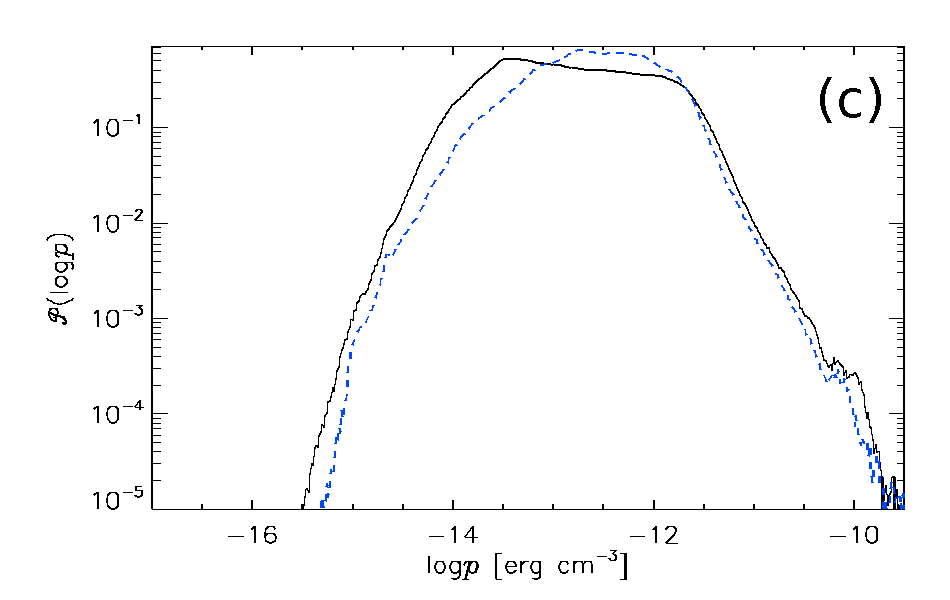
\includegraphics[width=0.9\columnwidth,clip=true,trim=0 0 0 9mm]{fig/o1pr_ppdf.png}
    \caption[Total volume probability distributions for Model~$\Ompa$ and $\Omph$]{
  Volume weighted probability distributions of gas number
  density~{\textbf{(a)}}, temperature~{\textbf{(b)}} and thermal
  pressure~{\textbf{(c)}} for  models {$\Omph$} (black, solid) and
  {$\Ompa$} (blue, dashed) for the total numerical domain $|z|\le1.12\kpc$.
    \label{fig:pdfm}}
  \end{figure}
%-----------------------------------------------------------------------------
  A three phase temperature distribution is visible for Model~$\Omph$ (HD)
  model in Fig.~\ref{fig:pdfm}b, while less apparent for Model~$\Ompa$ (MHD),
  with a significantly narrower range of temperatures.
  The bulk of the density distributions (a) are quite similar between the 
  HD and MHD model, except that the high densities are not as well resolved in
  the MHD model.
  The thermal pressure distributions are very similar, but with the HD modal
  pressure approximately one third the MHD modal pressure. 
  \footnote{FAG: I think these plots are averages of several snapshots in the 
  kinematic dynamo -- need to check -- while the analysis elsewhere is on the 
  saturated field}
  Even with a relatively weak magnetic field, there is significantly increased
  stiffness to the ISM, which restricts transport of the hot gas away from the
  disk \citep{Tomisaka98}, and may also act as a break on the supersonic
  flows, reducing the material collected in the snowplough phase of the SN and
  hence less cold gas resolved in the model \citep{Avillez04}
%-----------------------------------------------------------------------------
  \begin{figure}
  \centering
  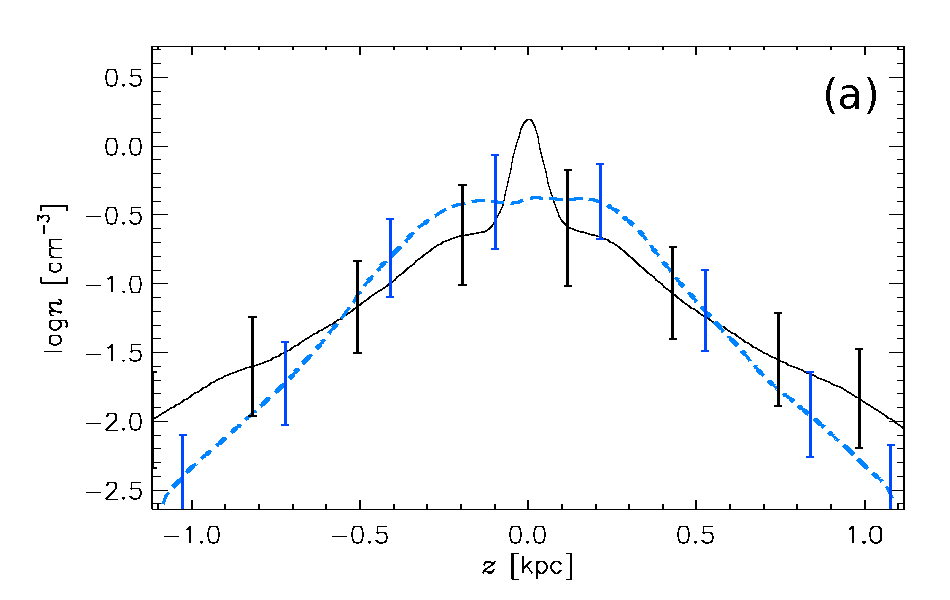
\includegraphics[width=0.9\columnwidth]{fig/zrhom.png}
  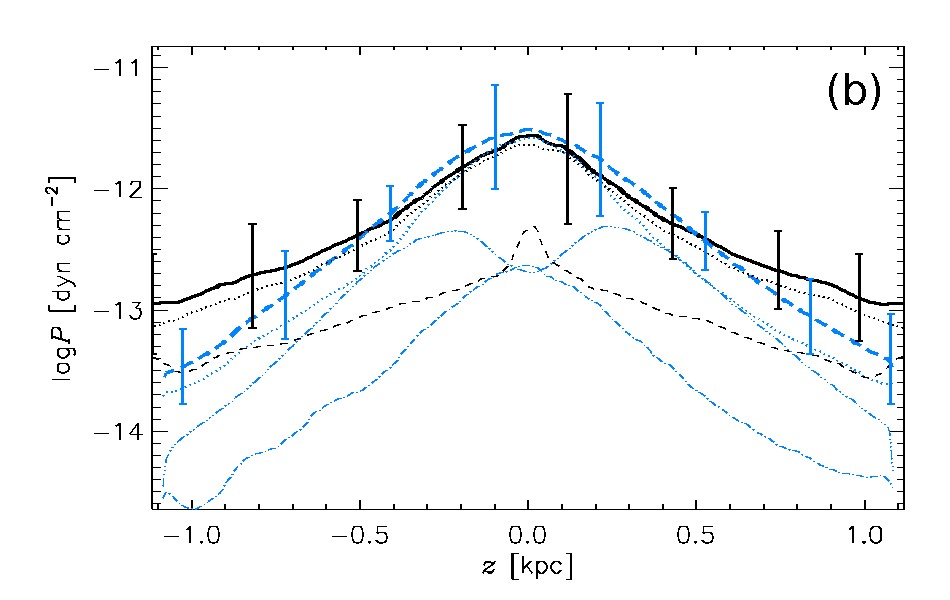
\includegraphics[width=0.9\columnwidth]{fig/zrppm.png}
    \caption[Horizontal averages of $n$ and $P$ for Model~$\Ompa$ and $\Omph$]{
  Horizontal averages of gas number density, $\mean{n}(z)$ {\textbf{(a)}}, and
  total pressure, $\mean{P}(z)$ {\textbf{(b)}}, for Model~{$\Ompa$} (solid,
  black), and Model~{$\Omph$} (dashed, blue). 
  Each are time-averaged using eleven snapshots respectively, spanning 
  100\Myr.
  The vertical lines indicate standard deviation within each horizontal slice.
  The thermal $\mean{p}(z)$ (dotted) and ram $\mean{p}\turb(z)$ (fine dashed)
  pressures are also plotted {\textbf{(b)}}.
%  For Model~{\OpH} the magnetic pressure $\mean{p}_B$ is also plotted (fine, 
%  dash-3dotted).
    \label{fig:zrhom}
            }
  \end{figure}
%-----------------------------------------------------------------------------

%  As discussed in Section~\ref{subsect:params} the stability of the disc
%  reduces the effectiveness of the SNe to generate and circulate hot gas, in
%  the absence of SN clustering. 
%  Hence Model~$\Omph$ has a slightly thicker disc, with less hot gas than 
%  Model~\Op.
  The effect of the magnetic pressure in Model~$\Ompa$ is to 
  expand the thick disc even further and this is illustrated in 
  Fig.~\ref{fig:zrhom}a, where the horizontal averages of gas number density
  $n(z)$ are plotted against $z$ for both models. 
  The strong peak in the density at the mid-plane is evident for Model~$\Omph$
  (black, solid), while for Model~$\Ompa$ (blue, dashed) there is a broad
  plateau in the density, extending to $|z|\simeq300\pc$, where the mean 
  magnetic field is strongest.
  
%-----------------------------------------------------------------------------
  \begin{figure}
  \centering
  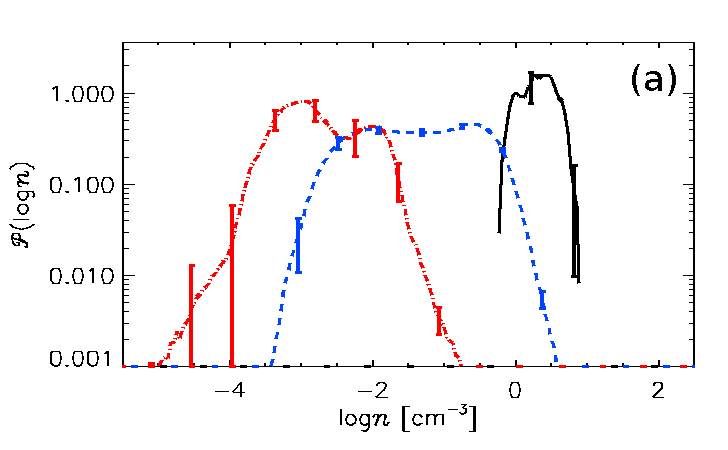
\includegraphics[width=0.9\linewidth]{fig/o1pr_npdf3s.png}  
  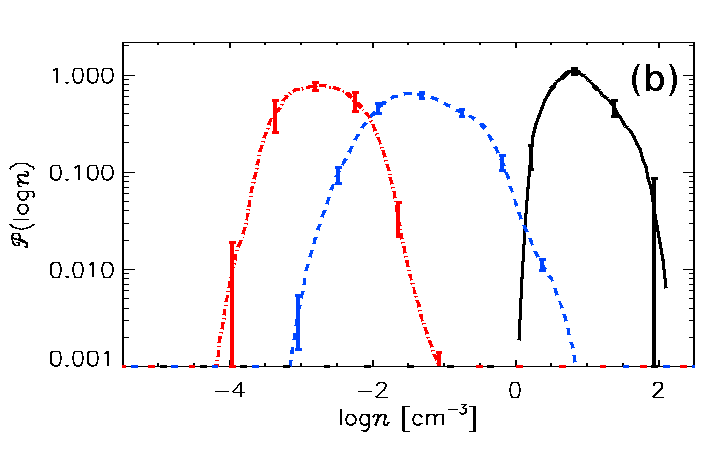
\includegraphics[width=0.9\linewidth]{fig/o1ph_npdf3s.png}\\  
  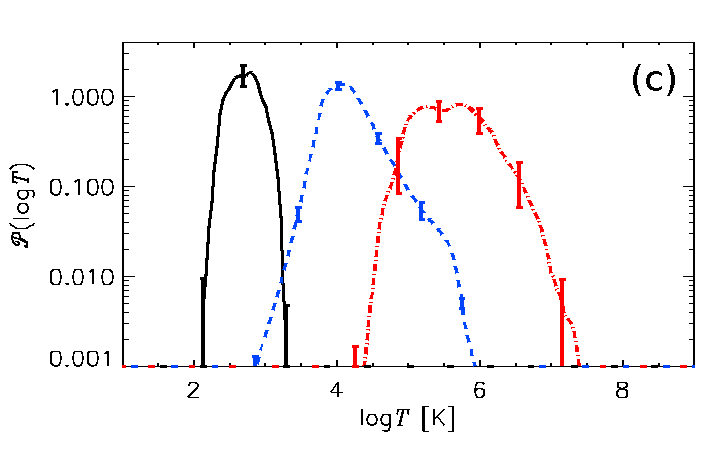
\includegraphics[width=0.9\linewidth]{fig/o1pr_tpdf3s.png}
  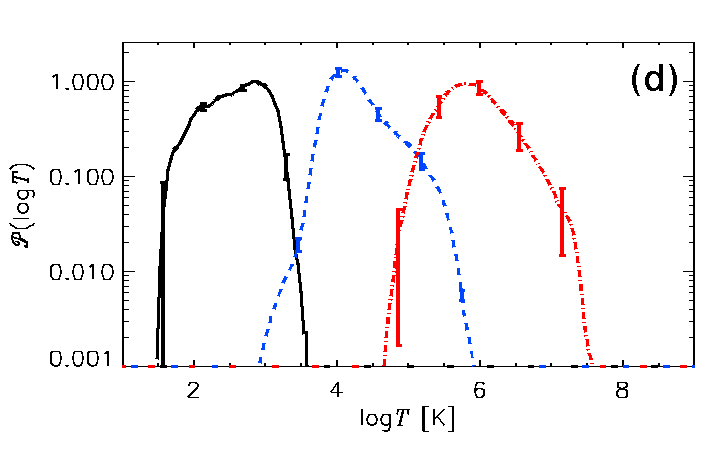
\includegraphics[width=0.9\linewidth]{fig/o1ph_tpdf3s.png}  
    \caption[Probability distributions by phase for $n$ and $T$]{
  Probability distributions by phase: cold (blue, dashed), warm (black, solid)
  and hot (red, dash-dotted) for gas number density ($n$ {\textbf{(a), (b)}})
  and temperature ($T$ {\textbf{(c), (d)}}) 
  for Model~$\Ompa$ ({\textbf{(a), (c)}}) and Model~$\Omph$
  ({\textbf{(b), (d)}}).
%  Data are averaged over 100\,Myr using eleven snapshots. 
  95\% confidence intervals for temporal deviation are shown as error bars.   
  \label{fig:npdf3s}
    }
  \end{figure}
%-----------------------------------------------------------------------------

  The horizontal averages of the pressure are plotted in Fig.~\ref{fig:zrhom}b
  for both models. 
  There is a strong peak at the mid-plane in the turbulent pressure for the HD
  model (black, dashed), but a much weaker profile for the MHD model (blue,
  dash-dotted). 
  There are two peaks in the magnetic pressure (blue, dash-3dotted) near 
  $|z|\simeq200\pc$, which supports the extended density profile.
  Another possible effect, which might constrain the circulation of the hot
  gas, and hence enhance the pressure at the mid-plane, is the strong 
  horizontal orientation of the field.
  The periodic boundary conditions
  exclude a non-zero vertical component to the mean field, so the magnetic
  tension predominantly acts against the vertical flows.
  Some understanding of the multi-phase structure of the magnetised ISM is
  still possible from these models, but the extreme temperatures and densities
  are significantly under represented.
  To improve this in future work it will be desirable to allow unrestricted 
  evolution of vertical field and to apply realistic clustering of the 
  SNe to generate more supperbubbles (composite multiple SN remnants forming a
  single superstructure) or chimneys (plumes venting hot gas from the disc 
  towards the halo).

  Results for separation of the ISM into three phases using the method 
  detailed in \cite[][Ch. 5.3]{Gent12} are shown for Models~$\Ompa$ and
  $\Omph$ in Fig~\ref{fig:npdf3s} with total volume probability distributions.
  The phases are defined using entropy $s$ such that for cold 
  $s<4.4\cdot10^{8}\erg \g^{-1}\K^{-1}$ and hot 
  $s>23.2\cdot10^{8}\erg \g^{-1}\K^{-1}$ with warm in between.
  Apart from the higher densities for the cold phase with the HD model (panel 
  b), 
  anticipated by the volume distributions (Fig.~\ref{fig:pdfm}), the warm and
  hot distributions for the MHD density (panel a) are broad, with a bimodal 
  structure to the hot gas. 
  The distributions for the warm gas (panels c and d) are very similar and for
  the cold (hot) distributions the MHD model does not extend to as low (high)
  temperatures. 
  
%-----------------------------------------------------------------------------
  \begin{figure}
  \centering
  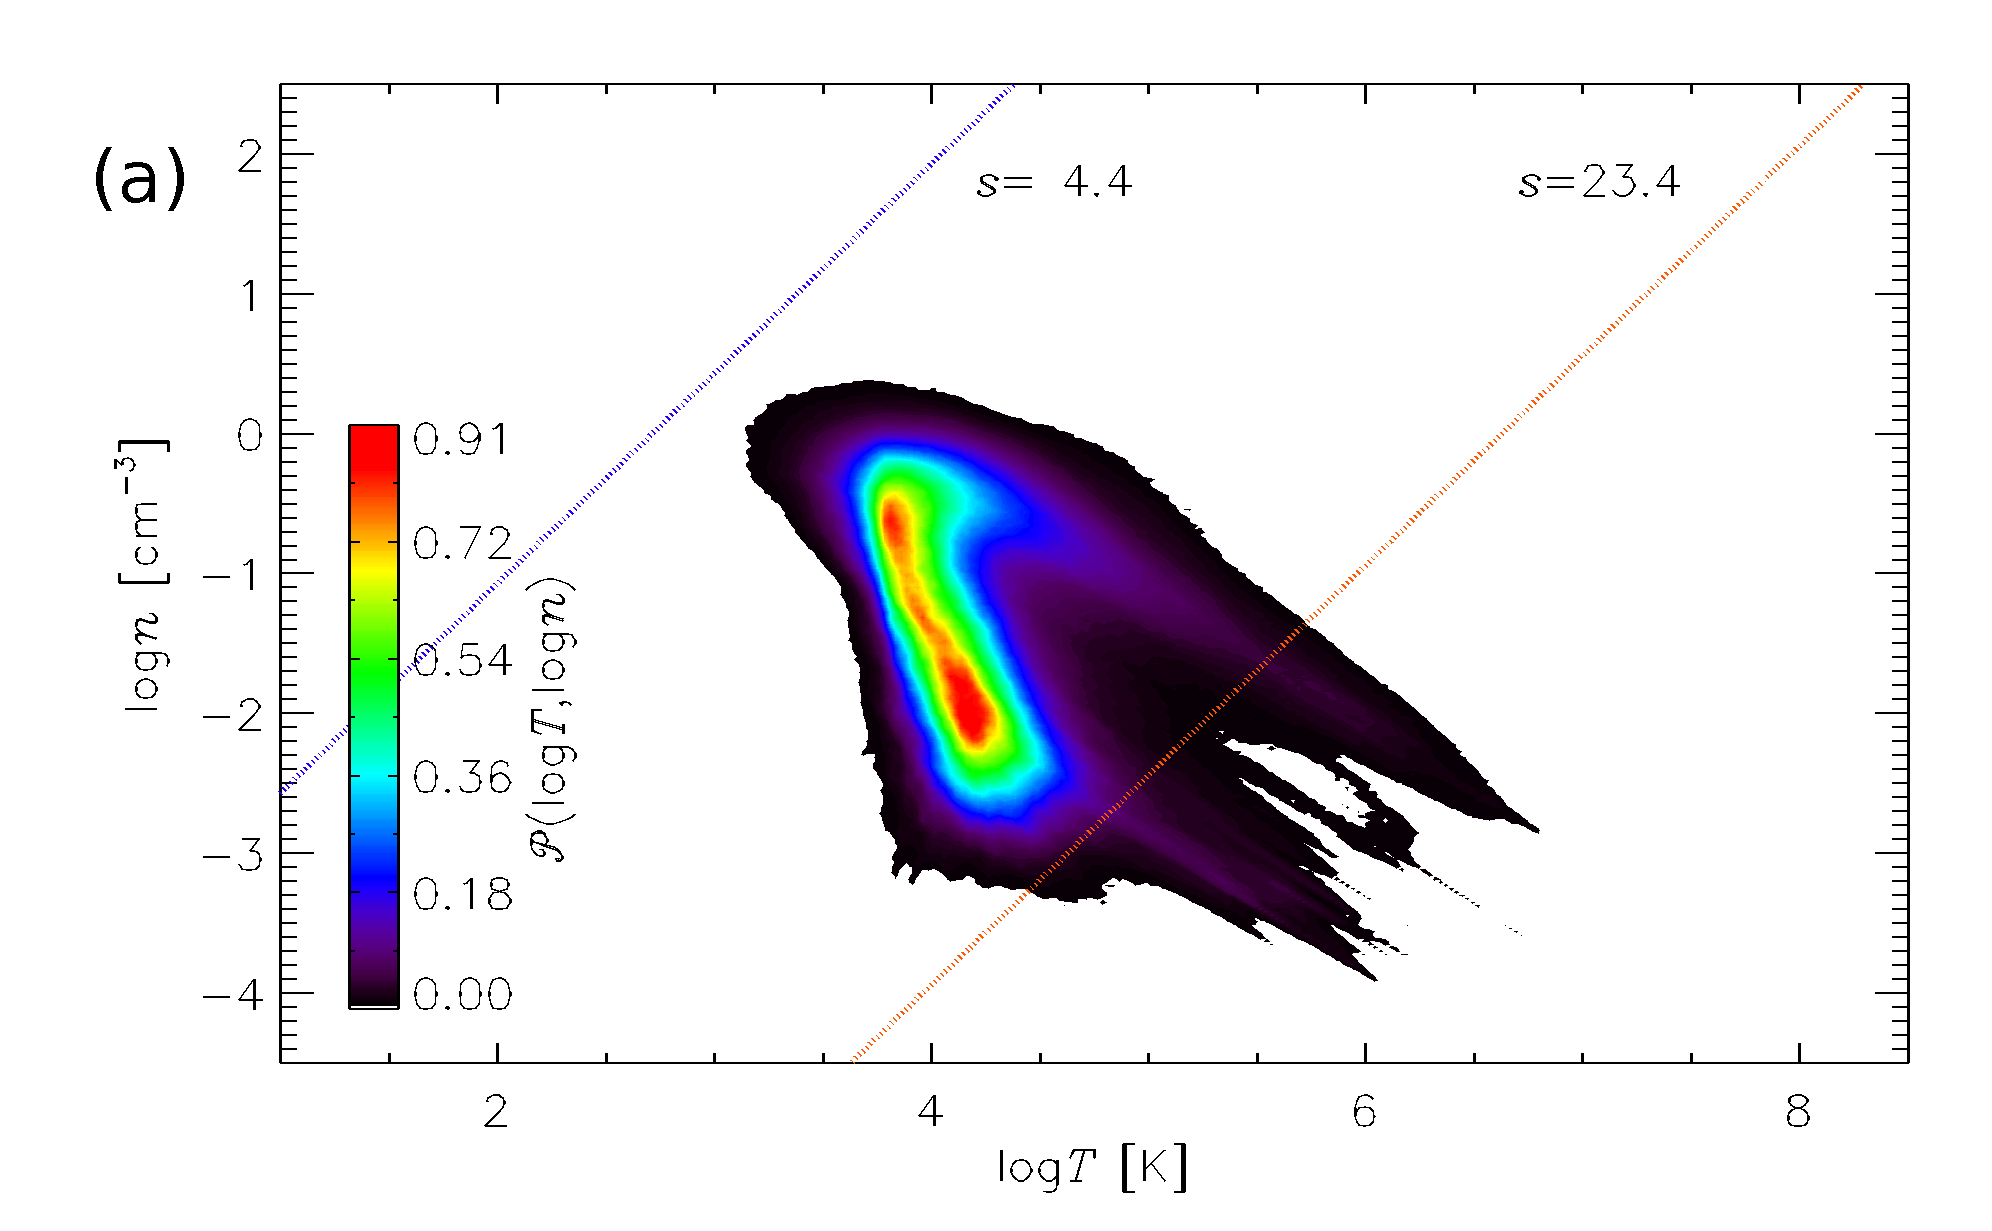
\includegraphics[width=0.9\linewidth]{fig/o1pr_pdf2dtn.png}  
  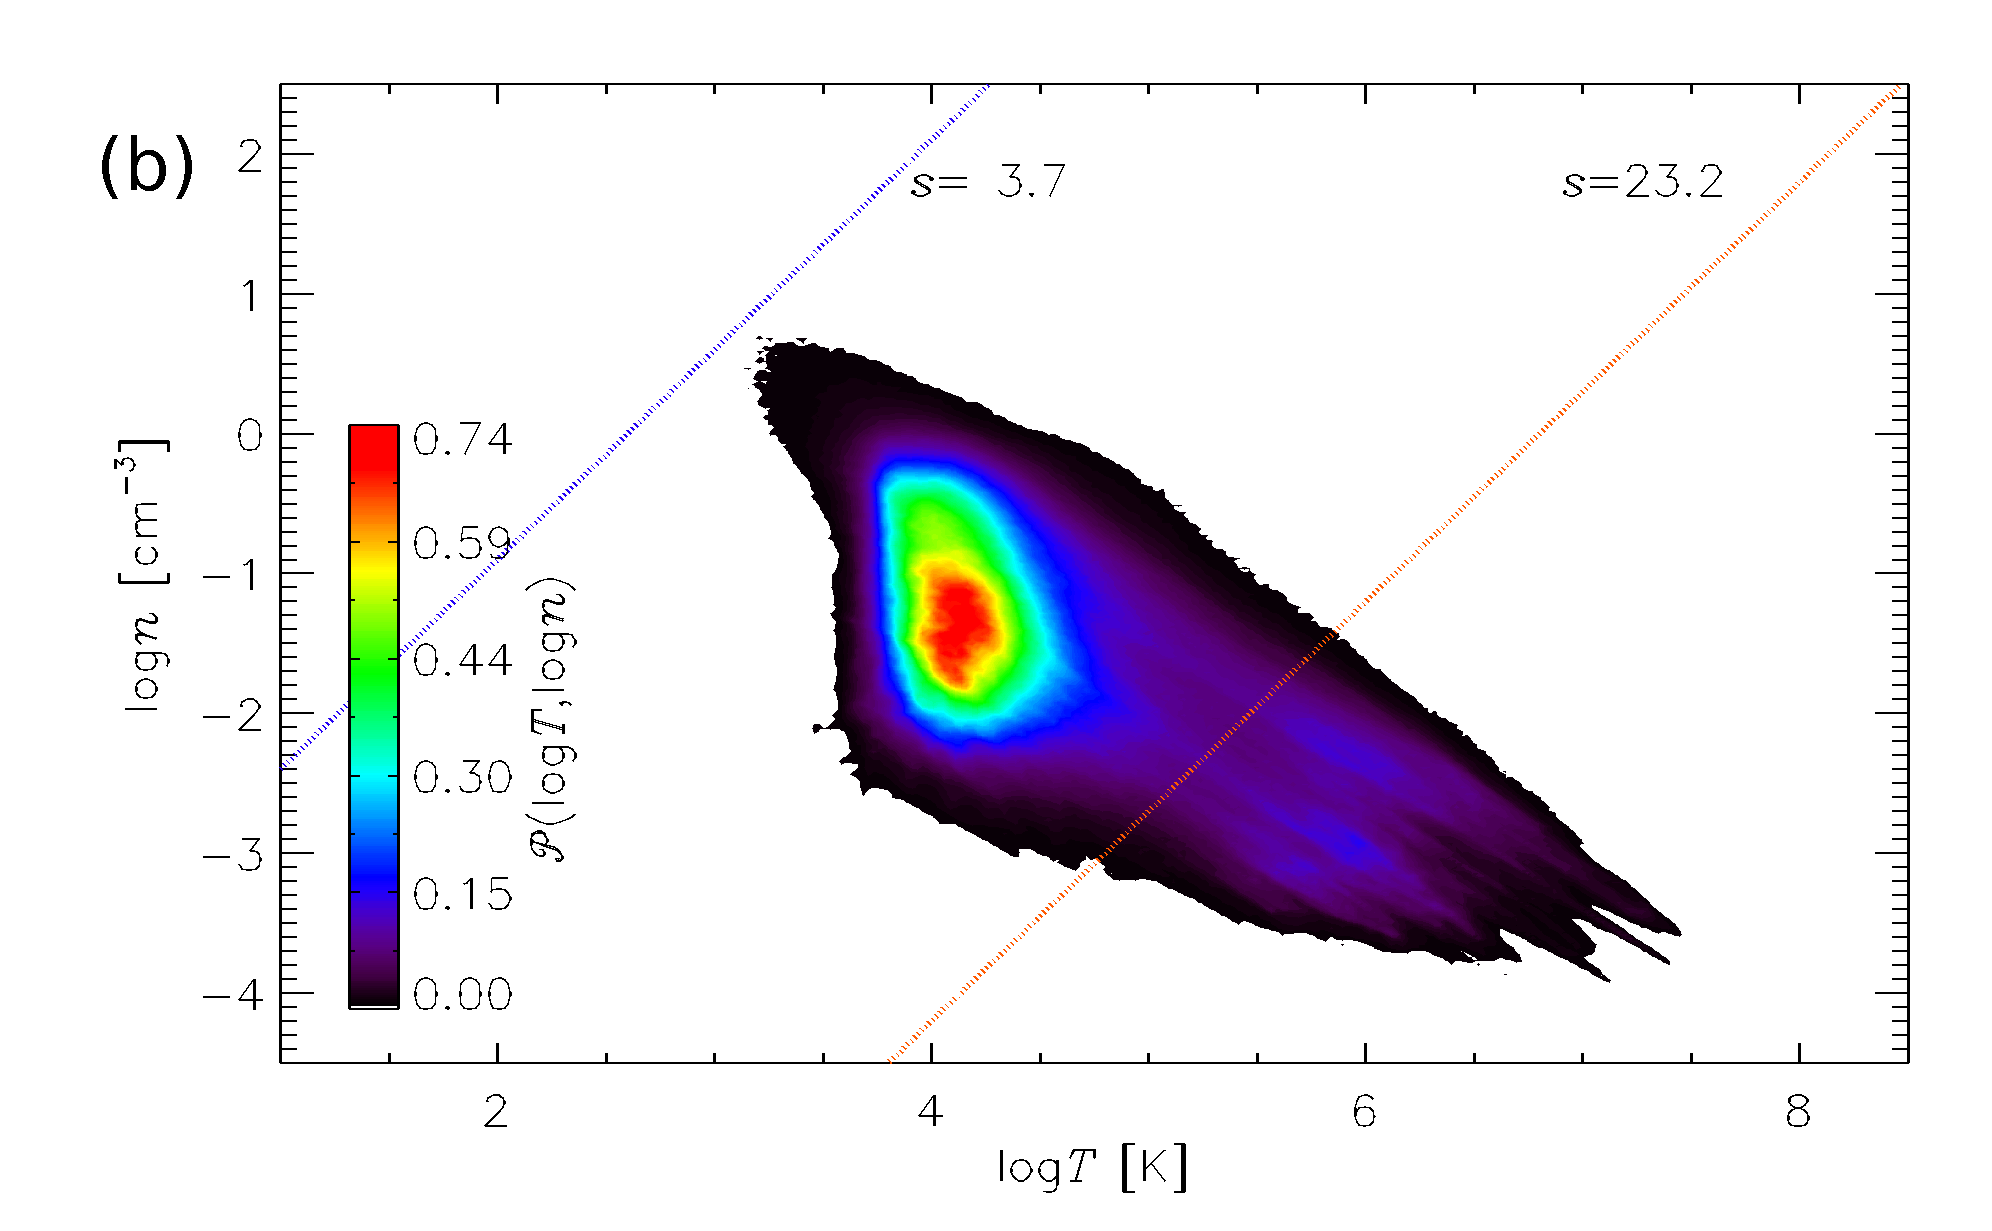
\includegraphics[width=0.9\linewidth]{fig/o1ph_pdf2dtn.png}
    \caption[2D probability distribution of $n$ and $T$ for Models~$\Ompa$ and $\Omph$]{
  Probability contour plot by volume of log$n$ vs log$T$ for Model~$\Ompa$
  {\textbf{(a)}}
  and Model~$\Omph$ {\textbf{(b)}}.
  The lines of constant entropy $s=4.4\cdot10^{8}$ 
  and $23.2\cdot10^{8}\erg\g^{-1}\K^{-1}$ indicate where the phases are defined
  as cold for $s\le4.4$ and as hot for $s>23.2$. 
  \label{fig:b2dv}
    }
  \end{figure}
%-----------------------------------------------------------------------------

  Comparing the combined probability distribution of density and temperature
  for both of these models in Fig.~\ref{fig:b2dv} with those of Model~\Op\
  in \cite[][Fig. 5.10]{Gent12} the spread is more broad and not obviously 
  aligned along a line of constant pressure.
  The HD distribution here is less compact than with MHD. 
  However when considering only the mid-plane distributions, as displayed in
  Fig.~\ref{fig:b2dh} the distributions match better with Model~\Op\ and the 
  pressure alignment is evident.
  So the broad distributions for the total volumes are explained by the 
  stronger gradient in the pressure distribution, due to the reduced 
  stirring of the hot gas.
  The thermal pressure at the mid-plane is also very similar in both models,
  reflected also in the agreement of the total and thermal pressure near the
  mid-plane in the plot of horizontal averages (Fig~\ref{fig:zrhom}b).
  The magnetic and turbulent pressure in Model~$\Ompa$ combine to match the
  mid-plane turbulent pressure alone of Model~$\Omph$.
  For the temperature in Model~$\Ompa$ the hot gas has two modes, evident in 
  Fig.~\ref{fig:b2dv}a at $10^5\K$ and $10^6\K$, but at the mid-plane there 
  only the single $10^3\K$ mode. 
  The structure of the ISM at the mid-plane is therefore common to both models
  with modes at $10^6\K,~10^{-2}\cmcube$ and $10^4\K,~1\cmcube$.
  The cold gas is insufficiently resolved in Model~$\Ompa$ for comparison. 
  
%-----------------------------------------------------------------------------
  \begin{figure}
  \centering
  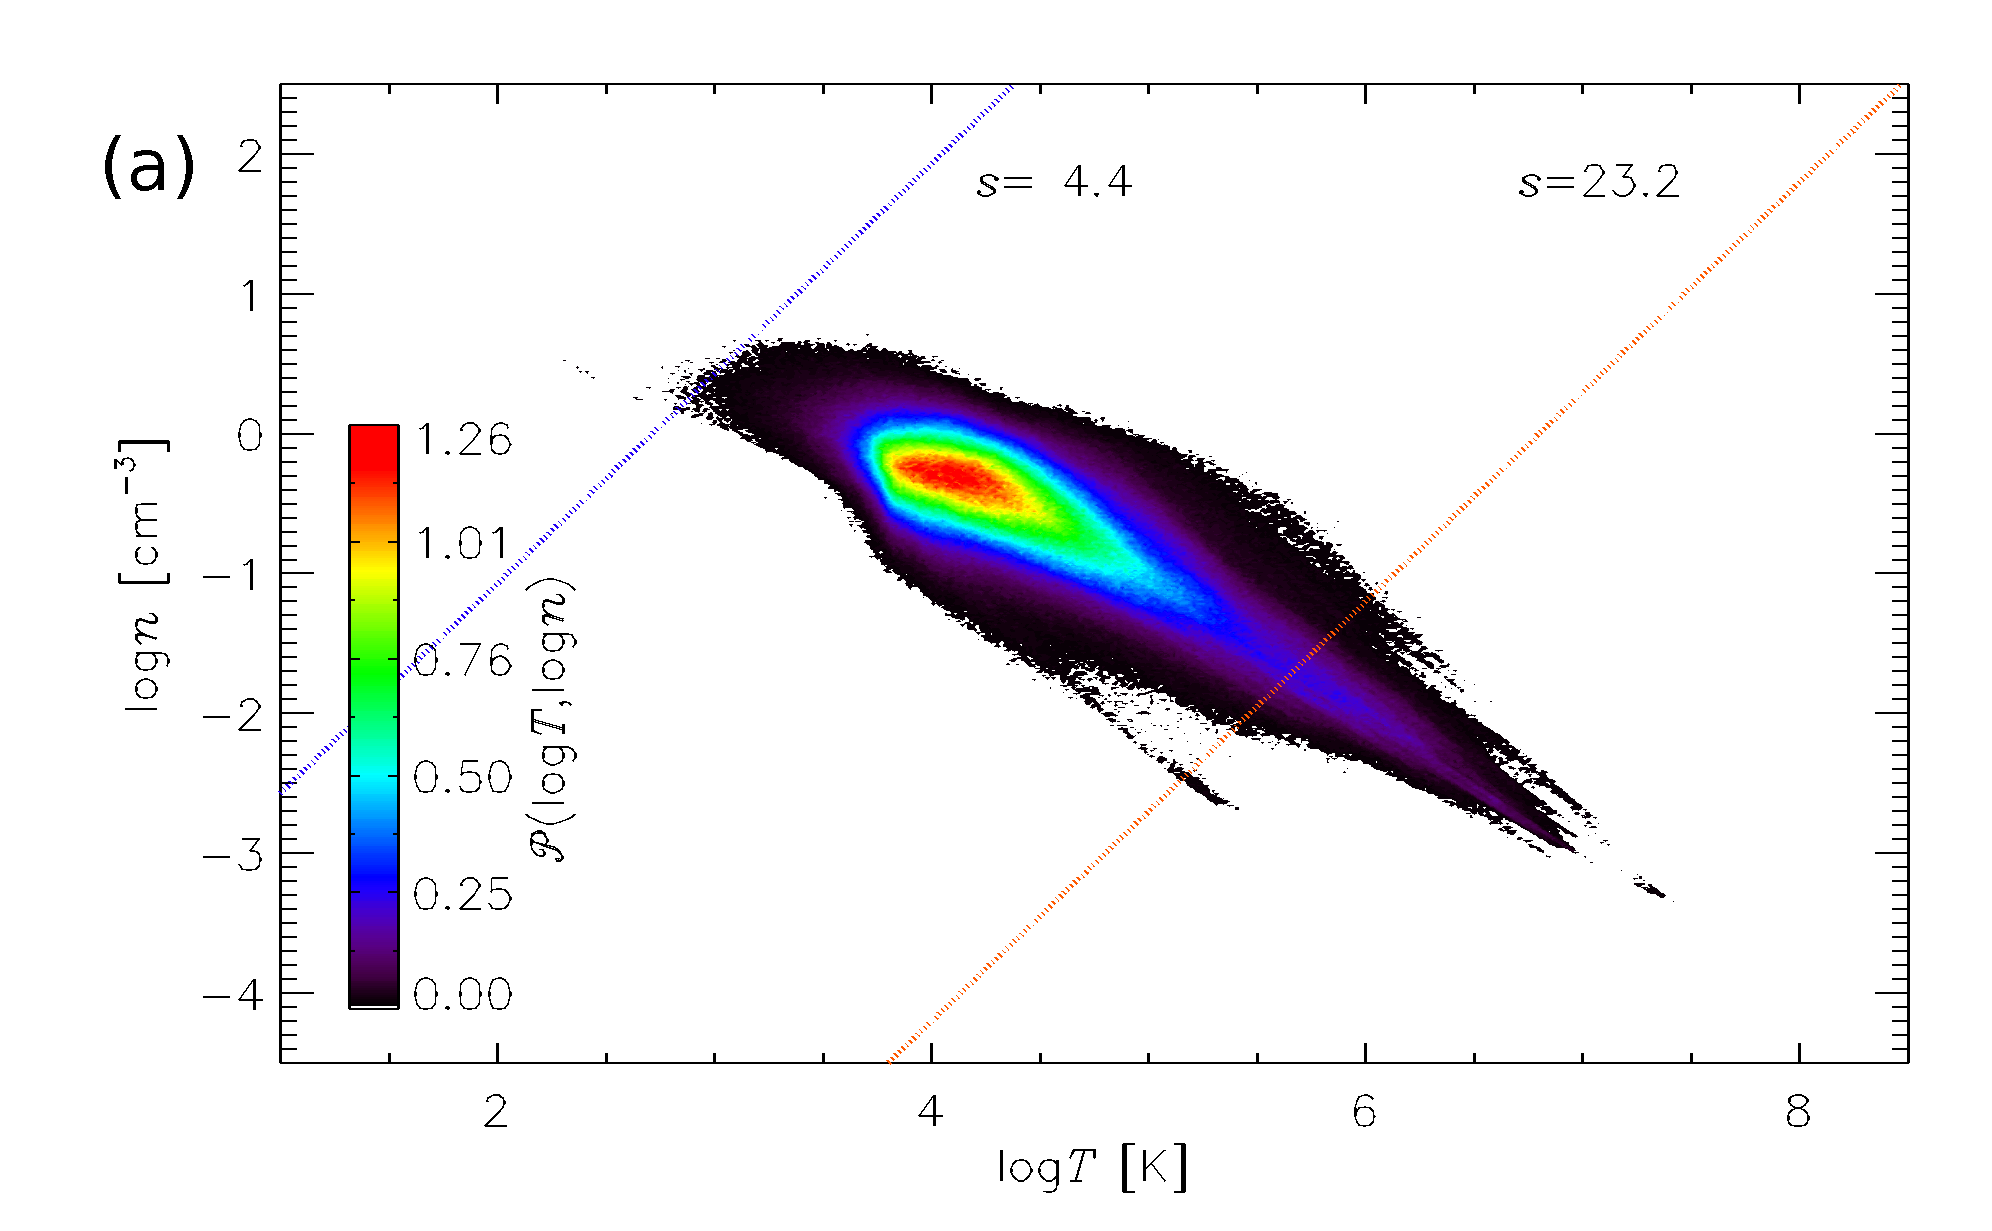
\includegraphics[width=0.9\linewidth]{fig/o1pr_pdf2dh.png}  
  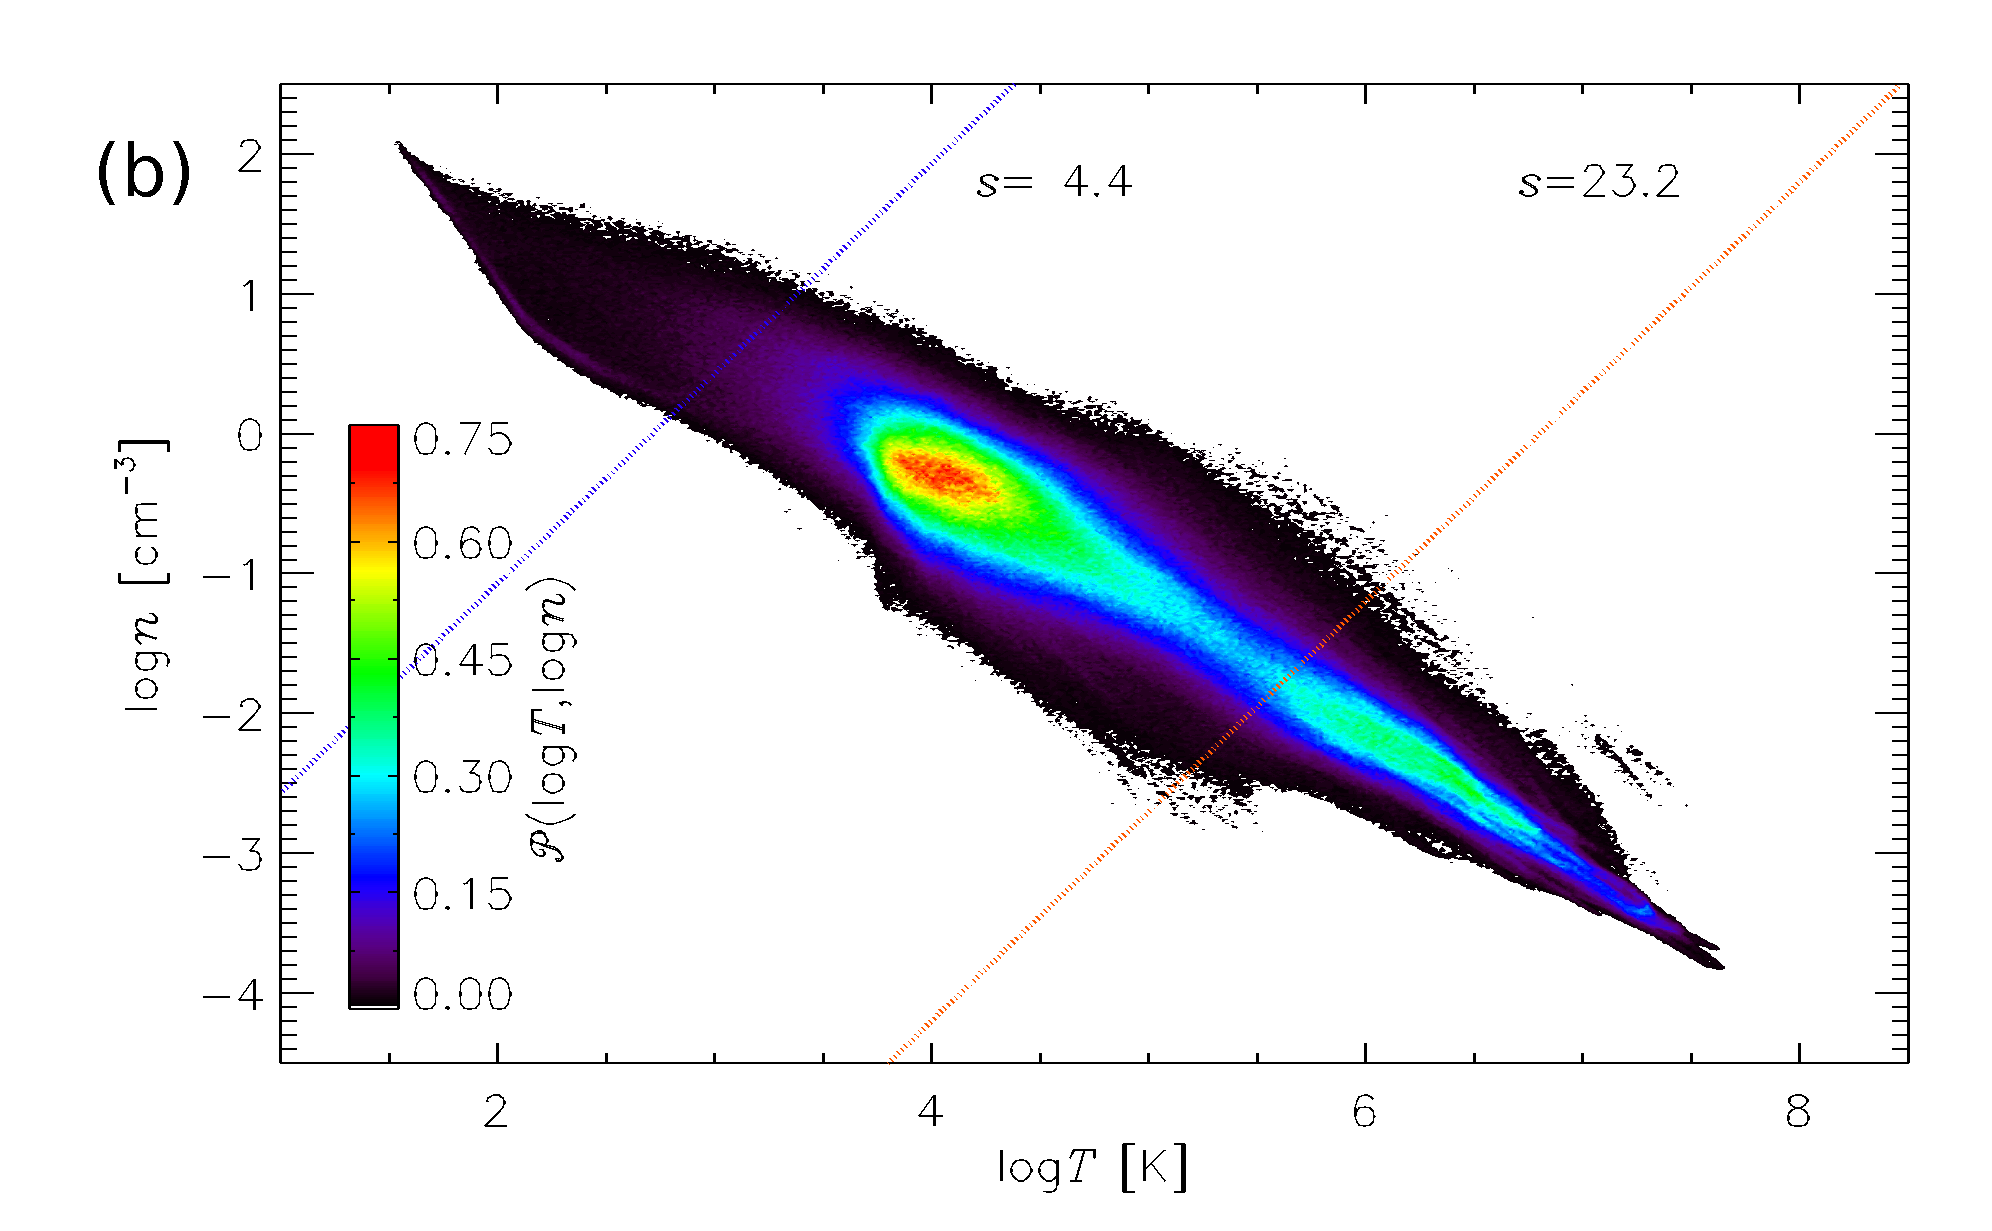
\includegraphics[width=0.9\linewidth]{fig/o1ph_pdf2dh.png}
    \caption[2D mid-plane probability distribution for Models~$\Ompa$ and  $\Omph$]{
  The mid-plane probability distributions ($|z|<100\pc$) by gas number density 
  $\log n$ and temperature $\log T$ for {\textbf{(a)}} Model~$\Ompa$ and
  {\textbf{(b)}} Model~$\Omph$.
  \label{fig:b2dh}
    }
  \end{figure}
%-----------------------------------------------------------------------------

  There is no evident dependence in the probability distributions between the 
  MHD models differing in rotation, shear or SN rate.
  The models in the kinematic stage extend to lower densities and higher 
  temperatures than either the HD Model~$\Omph$ or the MHD models in the 
  dynamo saturated state, and also extend to lower pressures.
  
%-----------------------------------------------------------------------------
  \begin{figure}
  \centering
  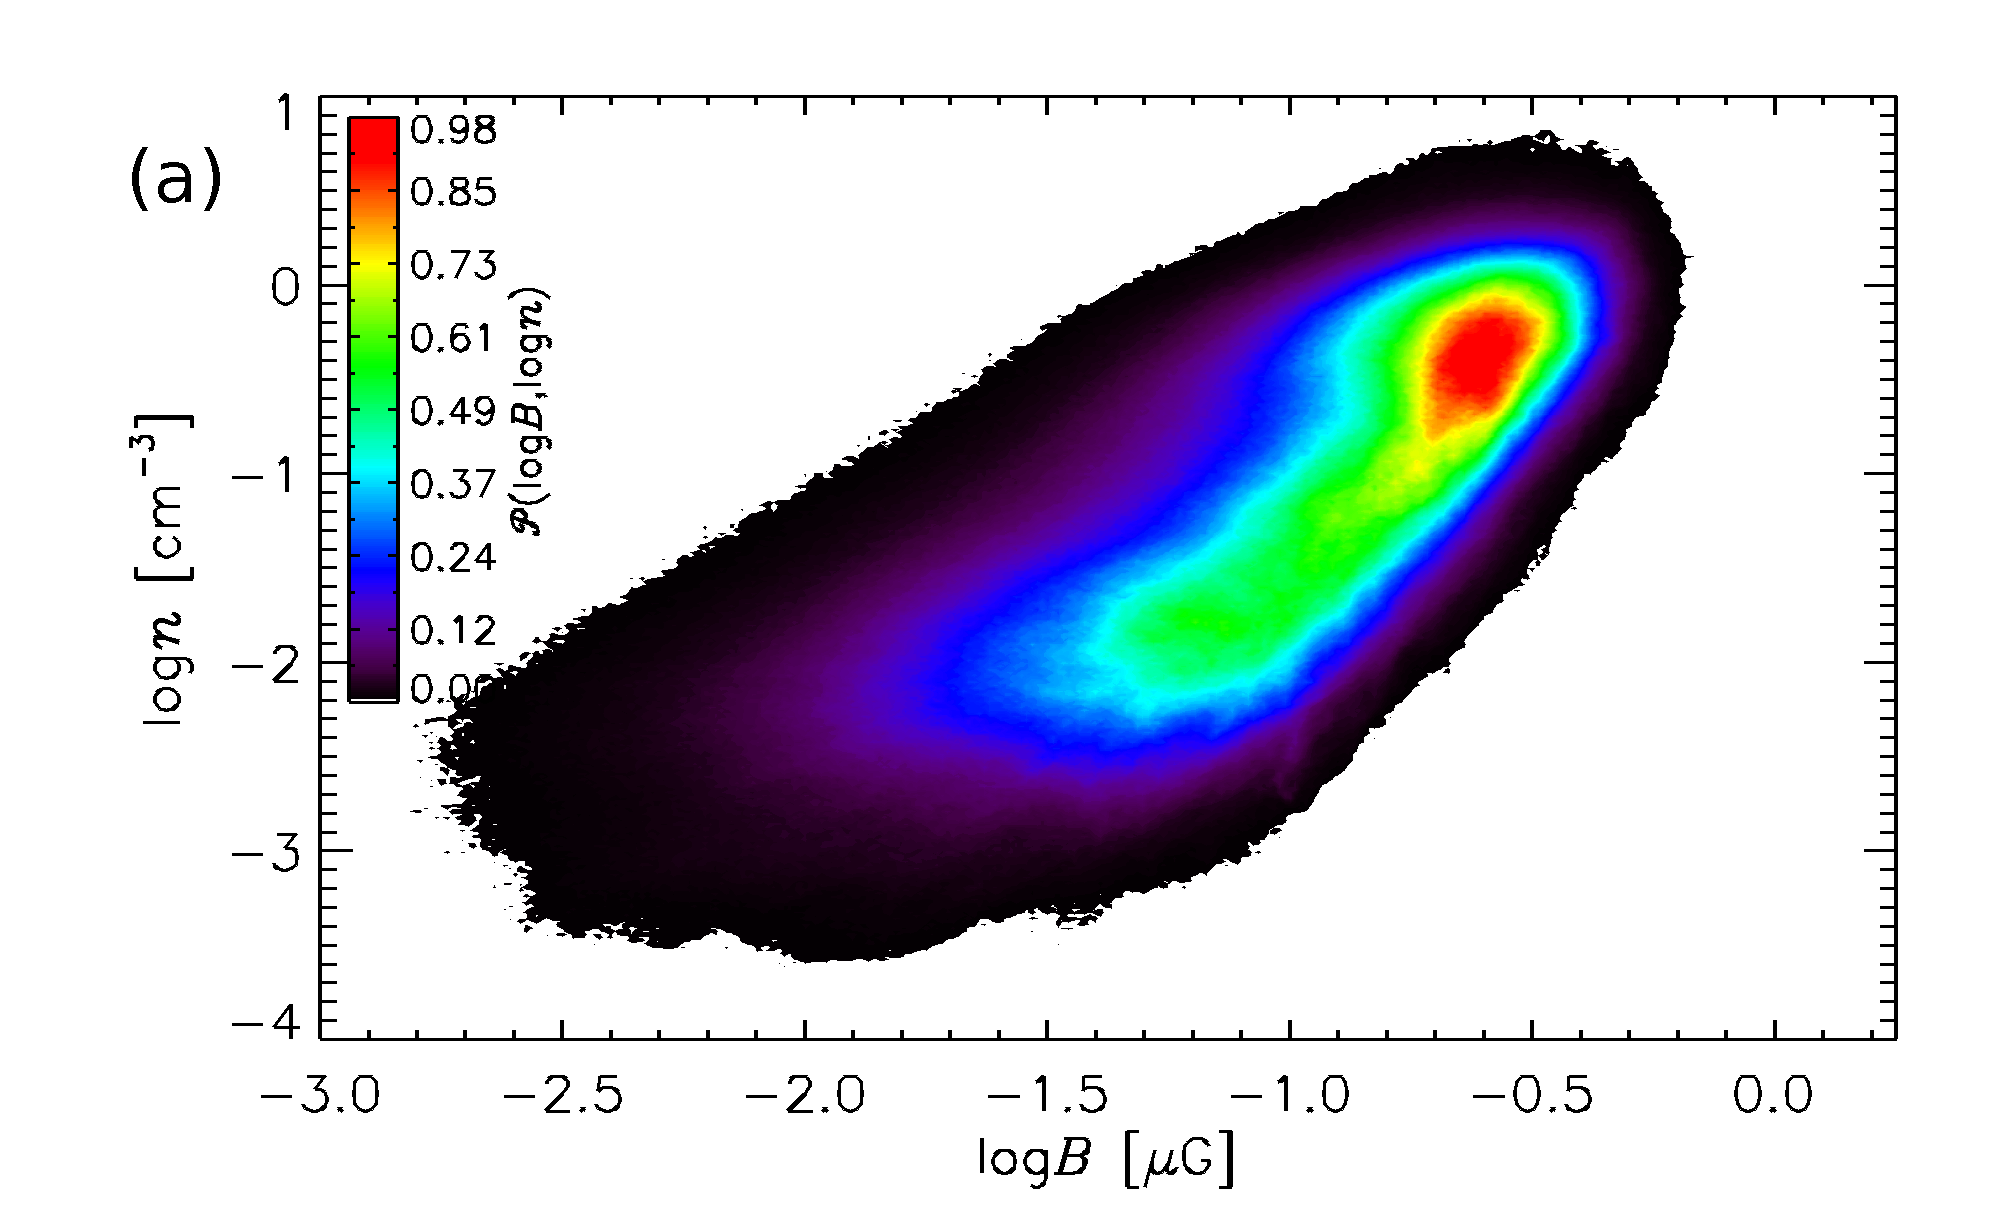
\includegraphics[width=0.9\linewidth]{fig/o1pr_pdf2db.png}  
  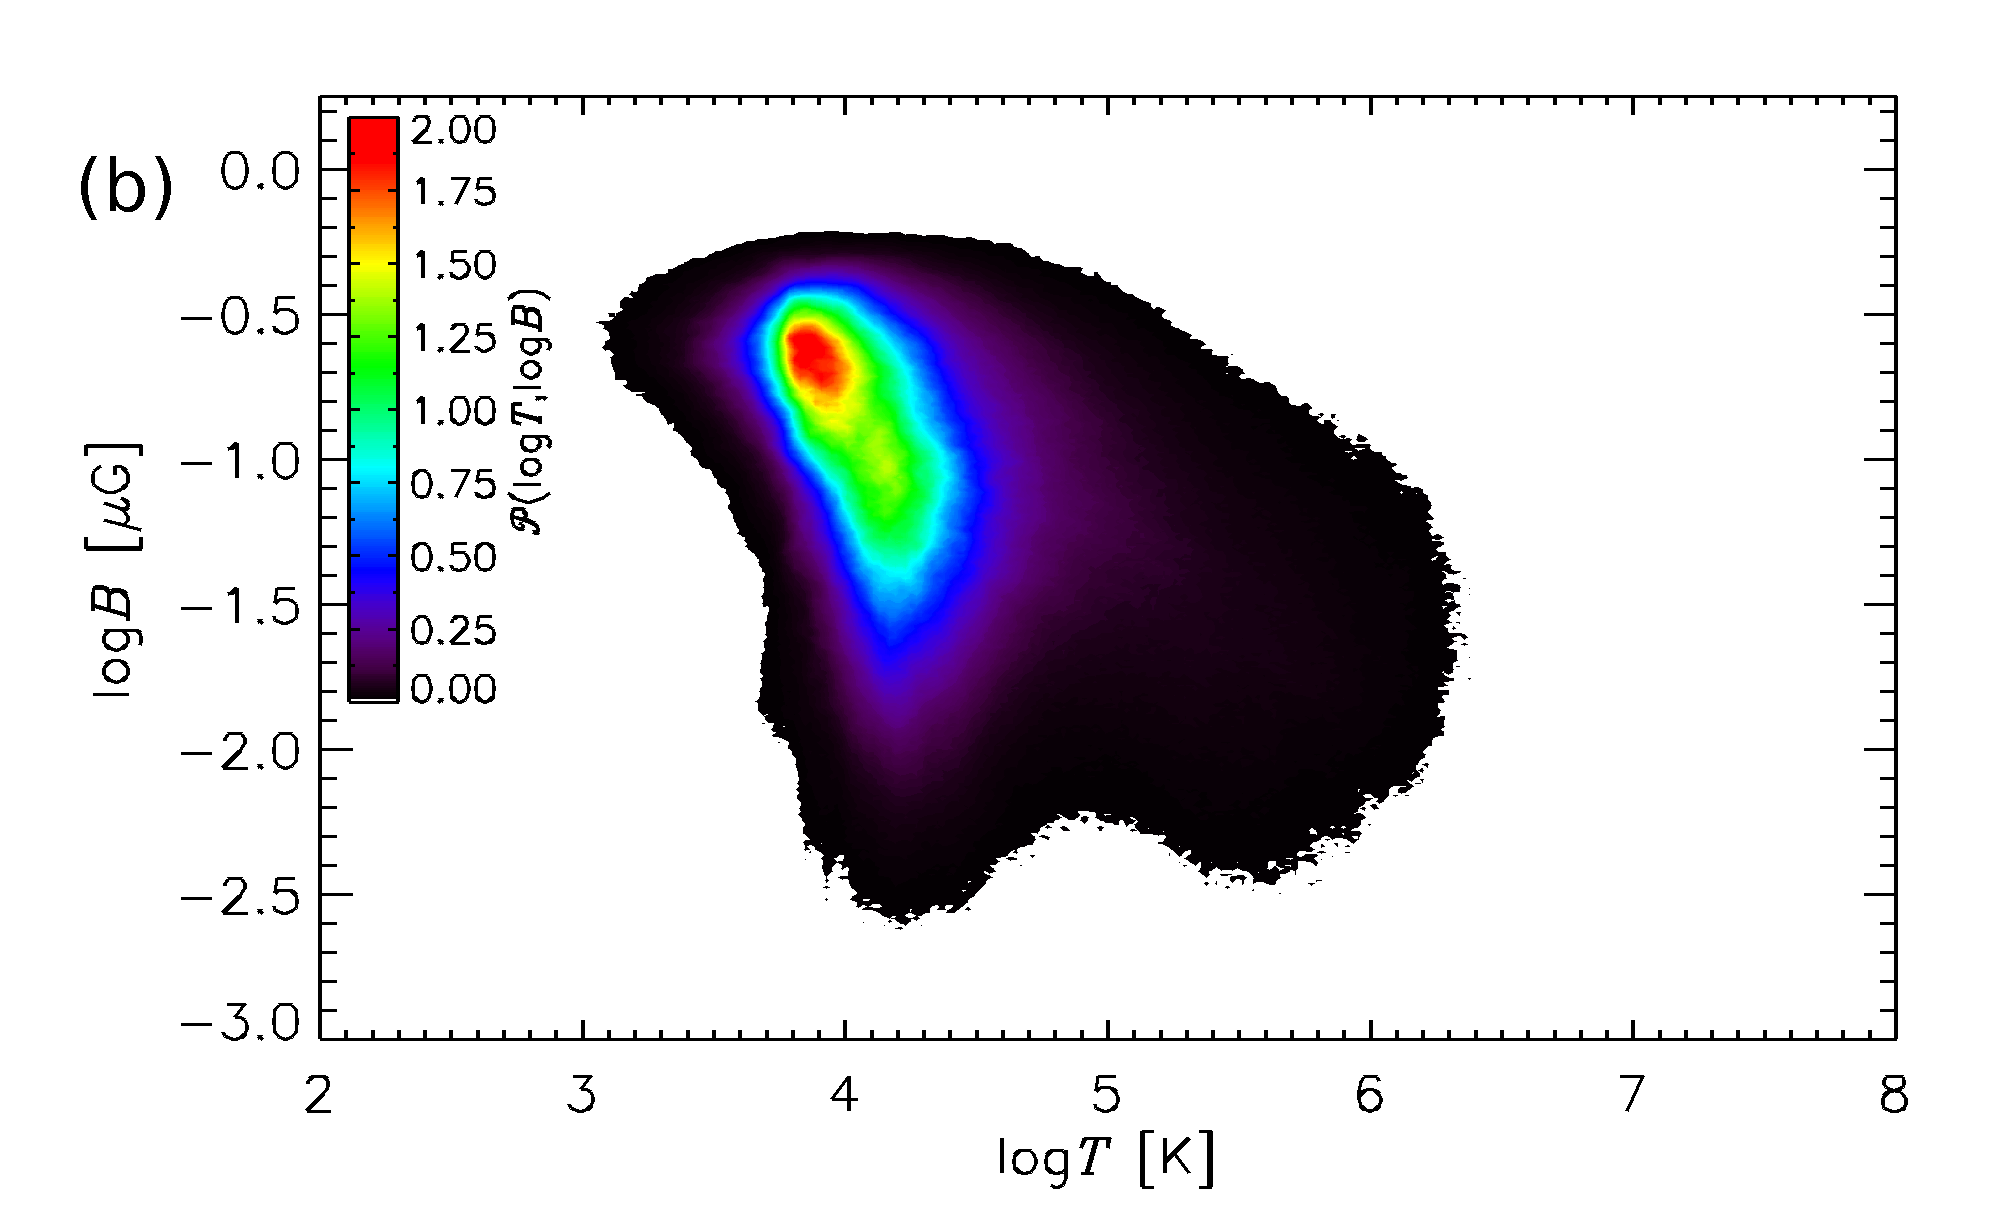
\includegraphics[width=0.9\linewidth]{fig/o1pr_pdf2tb.png}
    \caption[2D probability distribution of $n,B$ and $B,T$ for Model~$\Ompa$]{
  Total volume probability distributions ($|z|<100\pc$) by gas number density 
  $\log n$ and magnetic field strength $\log |B|$ {\textbf{(a)}} and
  temperature $\log |T|$ and magnetic field strength $\log |B|$ 
  {\textbf{(b)}} for Model~$\Ompa$.
  \label{fig:b2dnt}
    }
  \end{figure}
%-----------------------------------------------------------------------------

  In Fig.~\ref{fig:b2dnt}a the joint probability distributions of gas number 
  density with magnetic field strength is shown and in Fig.~\ref{fig:b2dnt}b
  of temperature with magnetic field strength for Model~$\Ompa$.
  From (a) it is clear there is a strong positive correlation between magnetic
  field strength and density and from (b) a weak negative correlation between
  temperature and field strength.
  The $T,B$ distribution has very strong peak at $T=10^4\K$.  
  
  
%-----------------------------------------------------------------------------
  \begin{figure*}
  \centering
  \hspace{-1.25cm}
  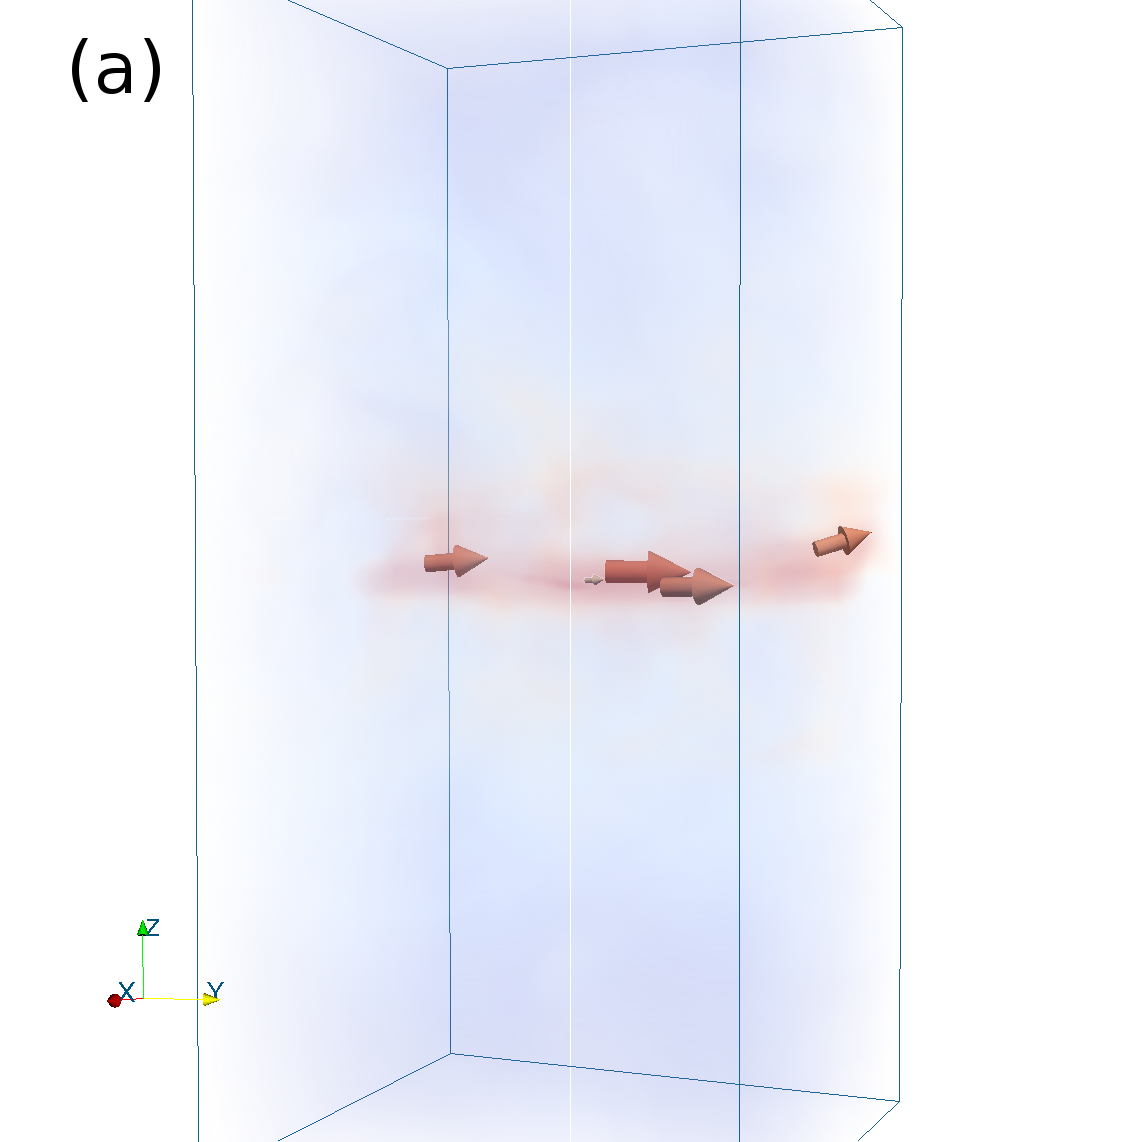
\includegraphics[width=0.35\linewidth]{fig/b310c.png}\hspace{-1.15cm}
  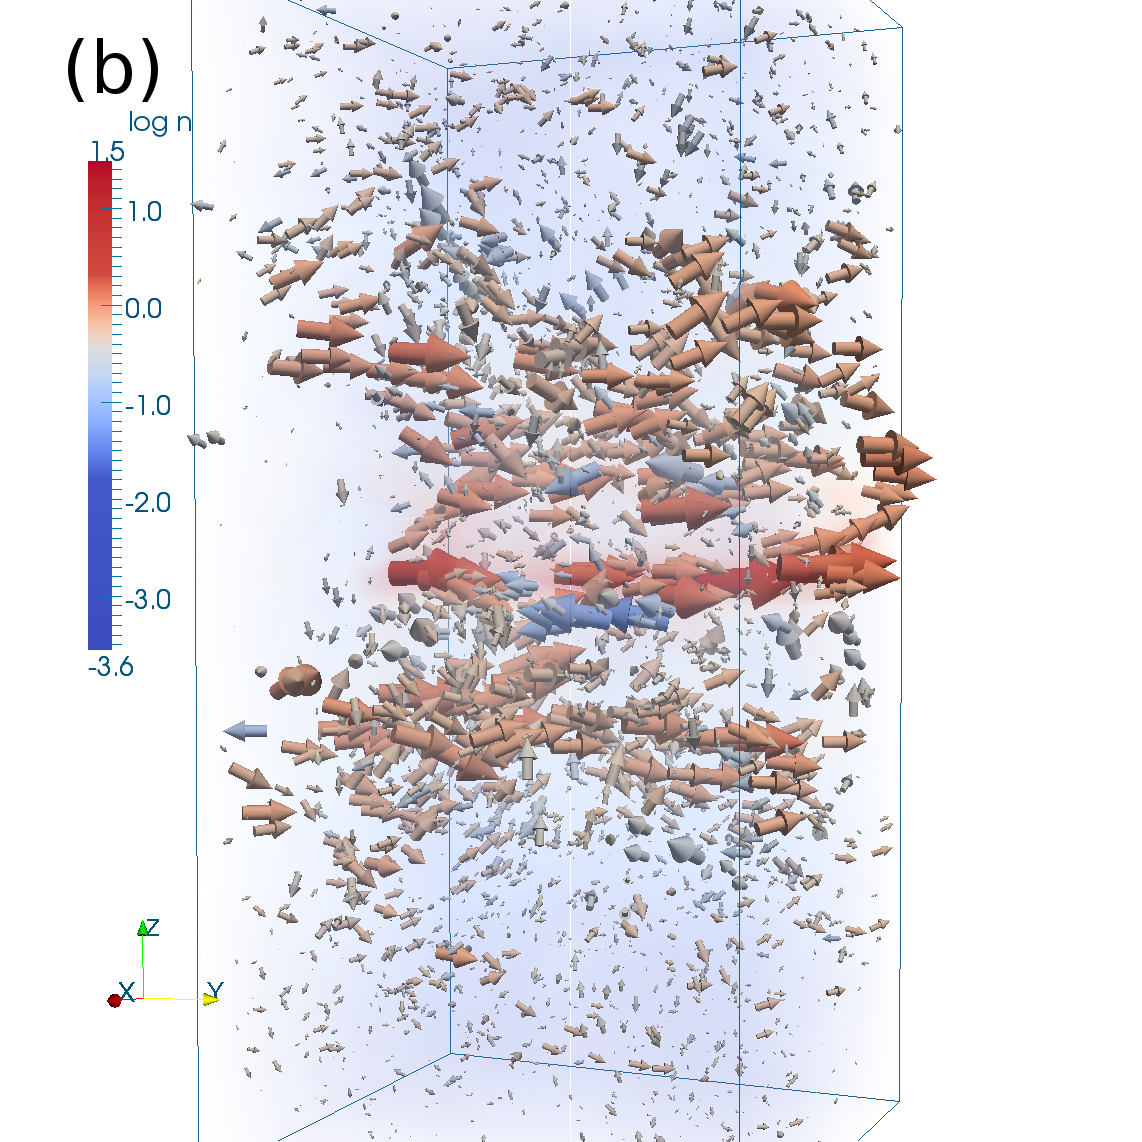
\includegraphics[width=0.35\linewidth]{fig/b310w.png}\hspace{-1.15cm}
  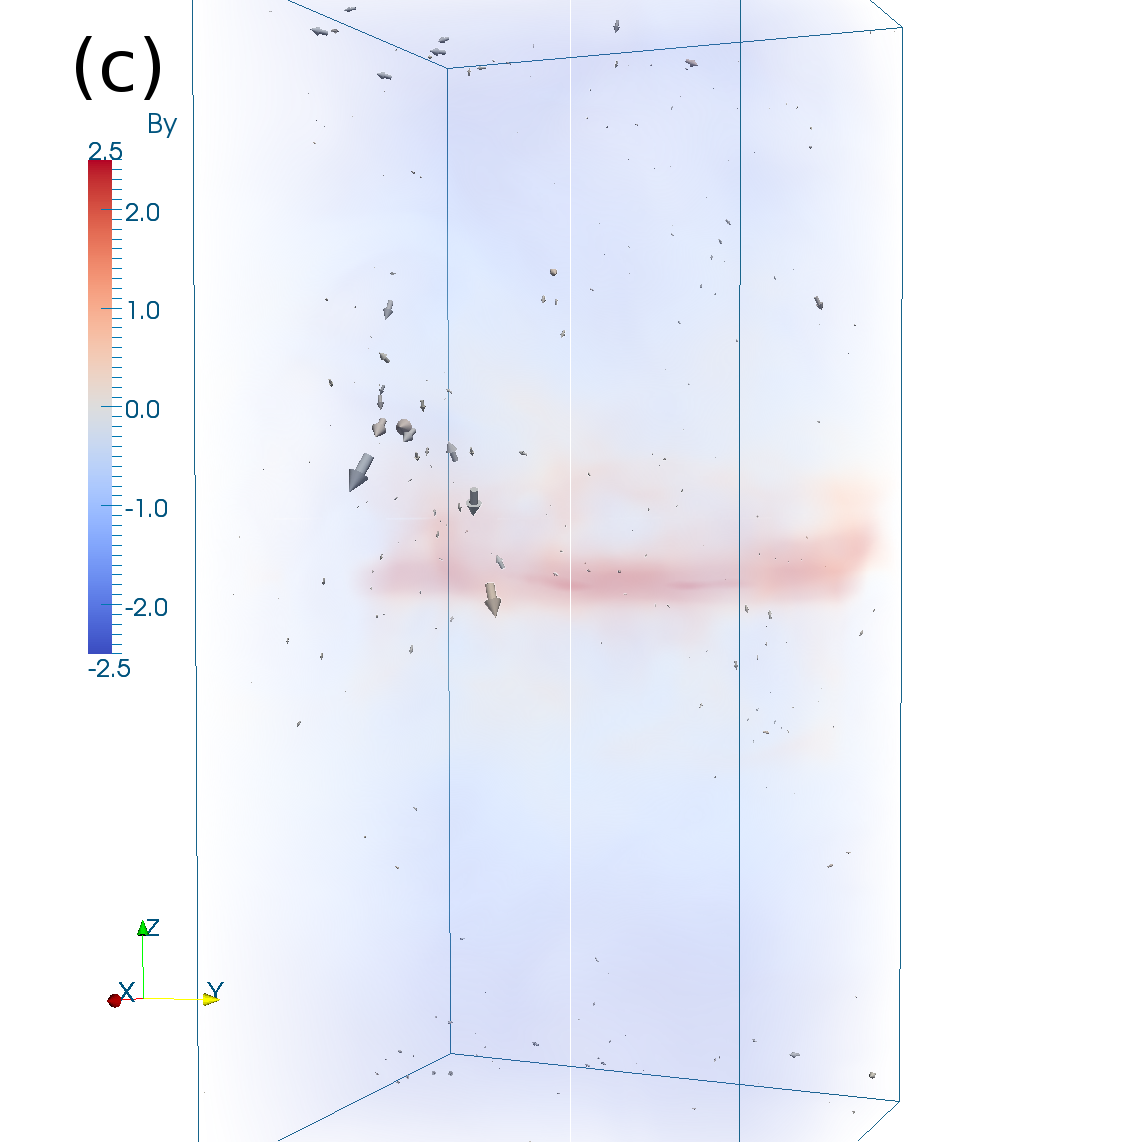
\includegraphics[width=0.35\linewidth]{fig/b310h.png}
  \hspace{-1.25cm}
  \caption[Volume snapshots of $\vect{B}$ by phase for Model~$\Ompa$]{
  Vector plots of the magnetic field $\vect{B}$ {\text{(a)}} in the cold phase
  {\text{(b)}} the warm phase and {\text{(c)}} the hot phase.
  Field directions are indicated by arrows and strength by their thickness.
  The colour of the arrows indicates the strength of the
  azimuthal ($y$) component (colour bar on the right).
  The background shading illustrates the density of the ISM.
  \label{fig:b3box}}
  \end{figure*}
%-----------------------------------------------------------------------------

  For Model~$\Ompa$ the ISM for a single snapshot is decomposed into the 
  three phases and the magnetic field for each plotted separately in 
  Fig.~\ref{fig:b3box}.
  In panel a the cold gas occupies only a limited volume near the mid-plane, 
  but the magnetic field is very strong and organised in alignment with the
  mean field surrounding it in the warm gas. 
  This is represented by the length and thickness of the vector arrows.  
  The colour of the arrows emphasises that the alignment has a strong 
  azimuthal component. 
  No arrows are present away from the mid-plane, because the cold gas is absent 
  there.
  In panel b the warm gas is present throughout the numerical volume.
  Field vectors are present almost throughout and the field is highly aligned,
  mainly in the azimuthal direction. 
  The strength of the field increases towards the mid-plane.
  The presence of some vectors in blue or grey indicates that there are 
  significant perturbations where the field includes reversals, some of these
  strong.
  Some of the field exhibits significant vertical orientation, but it is 
  mainly horizontal.
  In panel (c) the hot gas is also present throughout the volume, although 
  in smaller amounts near the mid-plane. 
  Despite this there is very little magnetic field.
  What field there is generally weak and lacks much systematic alignment, 
  although any orientation tends to be vertical, consistent with the
  field lines being stretched by the gas flowing away from the mid-plane. 
  Effectively the hot gas has a very weak field, which is highly disordered.
  Most of the magnetic field, and particularly the mean field, occupies the 
  warm gas.
  Detailed quantitative analysis of the structure of the gas will be deferred to
  future work.

%CCE - changed section to subsection after discussing with AS
  \subsection{Summary}
%CCE edit end
  The magnitude of the magnetic field is strongly aligned to the density of the
  ISM and indirectly the warm and cold phases.
  More particularly the mean field is stronger in the warm and cold gas, with 
  the hot gas containing a more random field. 
  The mean magnetic field and the magnetic energy is strongest at 
  $|z|\simeq300\pc$, just outside the SNe active region. 
  The fluctuating dynamo is likely to be strongest in this SNe active region,
  but due to the low magnetic Reynolds numbers in the simulations, it is likely
  that the field and energy is significantly weaker in the simulations than 
  might be expected.




